\chapter{Dasar Desain Schematic dan PCB}

\section{Tujuan}
\begin{enumerate}
    \item Belajar mendesain sirkuit elektronik menggunakan software
    \item Mengetahui fungsi setiap komponen dan cara implementasinya
    \item Memahami proses menyusun komponen agar bisa digunakan bersamaan dengan komponen lain untuk melakukan fungsi tertentu
    \item Untuk memperkenalkan beberapa konsep dasar dan teknik laboratorium dalam mendesain schematic dan PCB
    \item Mendesain rangkaian PCB yang nantinya dapat dicetak menjadi komponen dengan fungsi tertentu
\end{enumerate}


\section{Dasar Teori}
Sebelum menyusun hardware dan komponen kecil seperti IC di breadboard dan
bahkan mensoldernya di PCB, ada baiknya kita melakukannya di software terlebih dahulu agar
kita bisa mengecek kompatibilitas tiap komponen dan mengecekknya secara virtual
disamping secara rinci mengetahui fungsi setiap komponen yang hendak kita gunakan
nantinya. Pada praktikum kali ini akan digunakan software AutoCAD EAGLE untuk mendesain
schematic dan PCB yang nantinya akan diprint, selain memiliki fitur yang mumpuni, banyak
tutorial cara penggunaan serta tersedia banyak library komponen yang sering kali dipakai
pada project arduino, MCU, dan elektronika.

Praktikan diharapkan sudah membaca secara rinci modul instalasi EAGLE dan mencoba fitur-fitur dasarnya dengan membuat schematic sederhana. Pada kali ini praktikan
akan arahkan untuk membuat rangkaian schematic dan board menggunakan MCU esp-12f
dan beberapa komponen lain yang bisa diprogram menjadi alat IoT sederhana.

Kesalahan yang seringkali dijumpai pada proses desain PCB yaitu routing yang
membingunkan bagi pemula, atau jika sudah melakukan routing namun desainnya susah
dibaca oleh pengguna lain, maka dari itu untuk memudahkan pembacaan schematic
digunakanlah fitur name dan label, hal ini digunakan untuk menyederhanakan desain tanpa
mengurangi sedikitpun fungsi utama sirkuit tersebut. Untuk mengecek apakah komponen
tersebut telah terkoneksi, gunakan fitur SHOW dan arahkan kursor mouse ke arah kabel yang
ingin dicek, dan jika kabel pada ujung dan pangkal sama-sama ter-highlight maka komponen
yang mendapat suplai daya tersebut sudah pasti terkoneksi dengan benar.

\section{Tugas Pendahuluan}
\begin{enumerate}
    \item Baca dan pahami technical guide
    \item Pelajari semua datasheet dari semua IC yang digunakan pada percobaan ini!
    \item Buatlah schematic untuk output berupa nomor kelompok!
\end{enumerate}

\section{Alat dan Komponen}
\subsection{Alat}
\begin{enumerate}
    \item Laptop yang telah terinstall Autodesk Fusion 360
    \item Mouse
\end{enumerate}

\section{Eksperimen 1: Wiring Schematic Minimum System ESP8266}
Buatlah desain MINIMUM SYSTEM ESP8266 yang memiliki button untuk Reset dan
Flash. ESP8266 ini memerlukan JST 4 PIN yang akan disambungkan dengan USB to TTL untuk
memprogram chip. ESP8266 ini dapat digunakan dengan menggunakan tegangan 3,3V yang
nantinya akan dikontrol oleh voltage regulator yang dihubungkan dengan JST 2 PIN.

\begin{enumerate}
    \item Untuk memulai membuat Design klik “file” di kiri atas dan klik “New Electronics Design”
    lalu save (ctrl+s) dan beri nama “Minimum System ESP8266”.
        \begin{figure}[H]
            \centering
            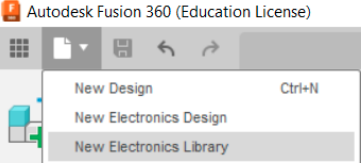
\includegraphics[width=0.6\linewidth]{P1/img/newelect.png}
            \caption{Buat Desain Baru} 
            \label{fig:buatdesainbaru}
        \end{figure}
    \item Selanjutnya untuk memulai mendesain schematic klik pada “New Schematic” lalu
    save (ctrl+s) dan beri nama “Schematic Minimum System ESP8266”.
        \begin{figure}[H]
            \centering
            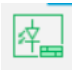
\includegraphics[width=0.16\linewidth]{P1/img/newschematic.png}
            \caption{Ikon New Schematic} 
            \label{fig:ikonnewschematic}
        \end{figure}
    \item Sebelum memulai mendesain pastikan library yang dibutuhkan sudah diunduh. Untuk
    mengupload library Workshop Telematika Buka tab “LIBARY” dan buka “Libary Manager”.
    Klik Pada “Import Library" dan pilih “Import From local Disk” lalu upload file library
    Workshop Telematika dengan file type .lbr
        \begin{figure}[H]
            \centering
            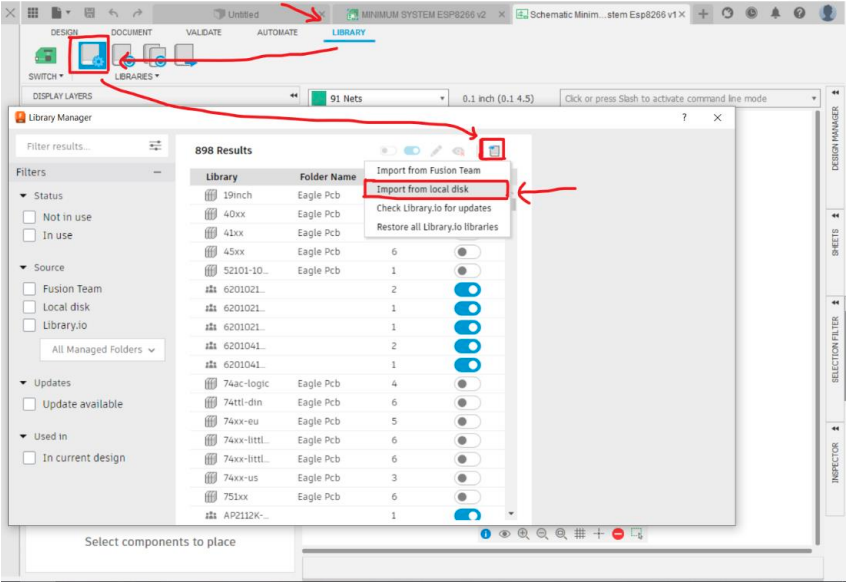
\includegraphics[width=0.7\linewidth]{P1/img/importLibrary.png}
            \caption{Library Fusion 360} 
            \label{fig:libraryfusion3601}
        \end{figure}
    komponen yang dibutuhkan adalah :
    \vspace{5pt}
    \begin{center}
        \vspace{-\topsep} % Mengurangi spasi sebelum tabel
        \begin{tabular}{|c|p{2cm}|m{2cm}|m{2cm}|m{2cm}|}
            \hline
            Gambar & Nama & Library & Jumlah & Catatan \\
            \hline
            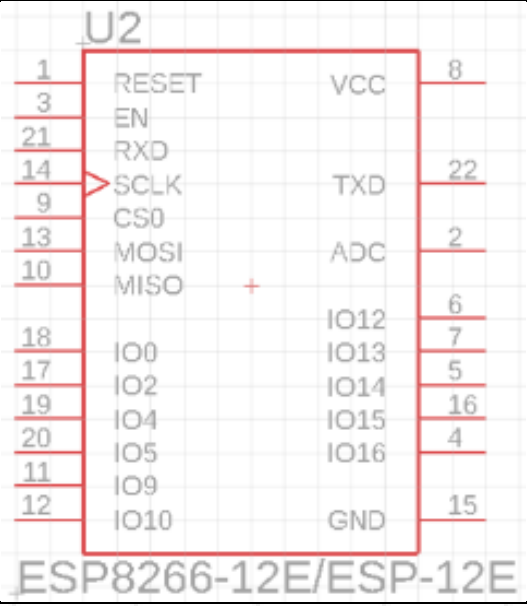
\includegraphics[width=0.2\linewidth]{P1/img/ESP8266.png} & ESP8266-
    12E/ESP-12E & Row 2, Col 3 & Row 2, Col 4 & Row 2, Col 5 \\
            \hline
            Row 3, Col 1 & Row 3, Col 2 & Row 3, Col 3 & Row 3, Col 4 & Row 3, Col 5 \\
            \hline
            Row 4, Col 1 & Row 4, Col 2 & Row 4, Col 3 & Row 4, Col 4 & Row 4, Col 5 \\
            \hline
            Row 5, Col 1 & Row 5, Col 2 & Row 5, Col 3 & Row 5, Col 4 & Row 5, Col 5 \\
            \hline
            Row 6, Col 1 & Row 6, Col 2 & Row 6, Col 3 & Row 6, Col 4 & Row 6, Col 5 \\
            \hline
            Row 7, Col 1 & Row 7, Col 2 & Row 7, Col 3 & Row 7, Col 4 & Row 7, Col 5 \\
            \hline
            Row 8, Col 1 & Row 8, Col 2 & Row 8, Col 3 & Row 8, Col 4 & Row 8, Col 5 \\
            \hline
            \end{tabular}
        \vspace{-\topsep} % Mengurangi spasi sebelum tabel
    \end{center}
    
    \vspace{5pt}
    \item Komponen dapat ditemukan dengan menggunakan tools \textbf{"Place Component"}
        \begin{figure}[H]
            \centering
            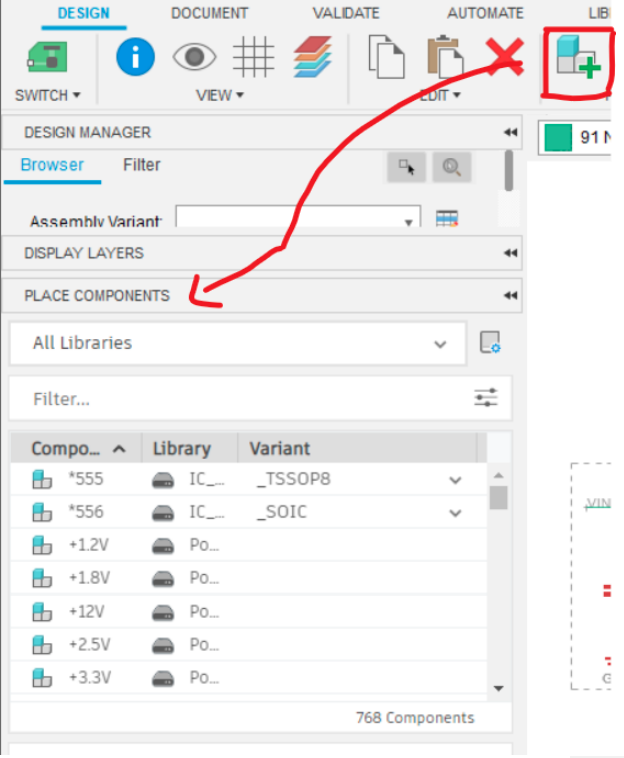
\includegraphics[width=0.7\linewidth]{P1/img/placecomponent.png}
            \caption{Place Component} 
            \label{fig:libraryfusion360}
        \end{figure}
    \item Untuk melakukan wiring atau koneksi pin gunakan Tools \textbf{Net} 
        \begin{figure}[H]
            \centering
            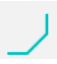
\includegraphics[width=0.2\linewidth]{P1/img/net.png}
            \caption{Tools Net} 
            \label{fig:toolsnet}
        \end{figure}
    koneksi yang diperlukan adalah :
    \begin{enumerate}
        \item 3,3-VOLTAGE-REGULATOR GND <-> JST 2 PIN GND / GND
        \item 3,3-VOLTAGE-REGULATOR VIN/IN <-> JST 2 PIN VCC
        \item 3,3-VOLTAGE-REGULATOR VIN/IN <-> Capacitor (1) <-> JST 2 PIN GND / GND
        \item 3,3-VOLTAGE-REGULATOR VOUT/OUT <-> Capacitor (2) <-> JST 2 PIN GND / GND
        \item 3,3-VOLTAGE-REGULATOR VEN/EN <-> JST 2 PIN VCC
        \item ESP8266 GND <-> JST 2 PIN GND / GND
        \item ESP8266 VCC <-> 3,3-VOLTAGE-REGULATOR VOUT/OUT
        \item ESP8266 GPIO15 <-> Resistor (1) <-> JST 2 PIN GND / GND
        \item ESP8266 EN/CH-PD <-> Resistor (2) <-> 3,3-VOLTAGE-REGULATOR VOUT/OUT
        \item ESP8266 RST/RESET <-> Resistor (3) <-> 3,3-VOLTAGE-REGULATOR VOUT/OUT
        \item ESP8266 RST/RESET <-> Switch (1) <-> JST 2 PIN GND / GND
        \item ESP8266 GPIO0 <-> Resistor (4) <-> 3,3-VOLTAGE-REGULATOR VOUT/OUT
        \item ESP8266 GPIO0 <-> Switch (2) <-> Resistor (5) <-> JST 2 PIN GND / GND
        \item ESP8266 RXD <-> JST 4 PIN RXD
        \item ESP8266 TXD <-> JST 4 PIN TXD
        \item JST 4 PIN VCC <-> 3,3-VOLTAGE-REGULATOR VOUT/OUT
        \item JST 4 PIN GND <-> JST 2 PIN GND / GND
    \end{enumerate}
\end{enumerate}
\textbf{Referensi rangkaian:}
\begin{figure}[H]
    \centering
    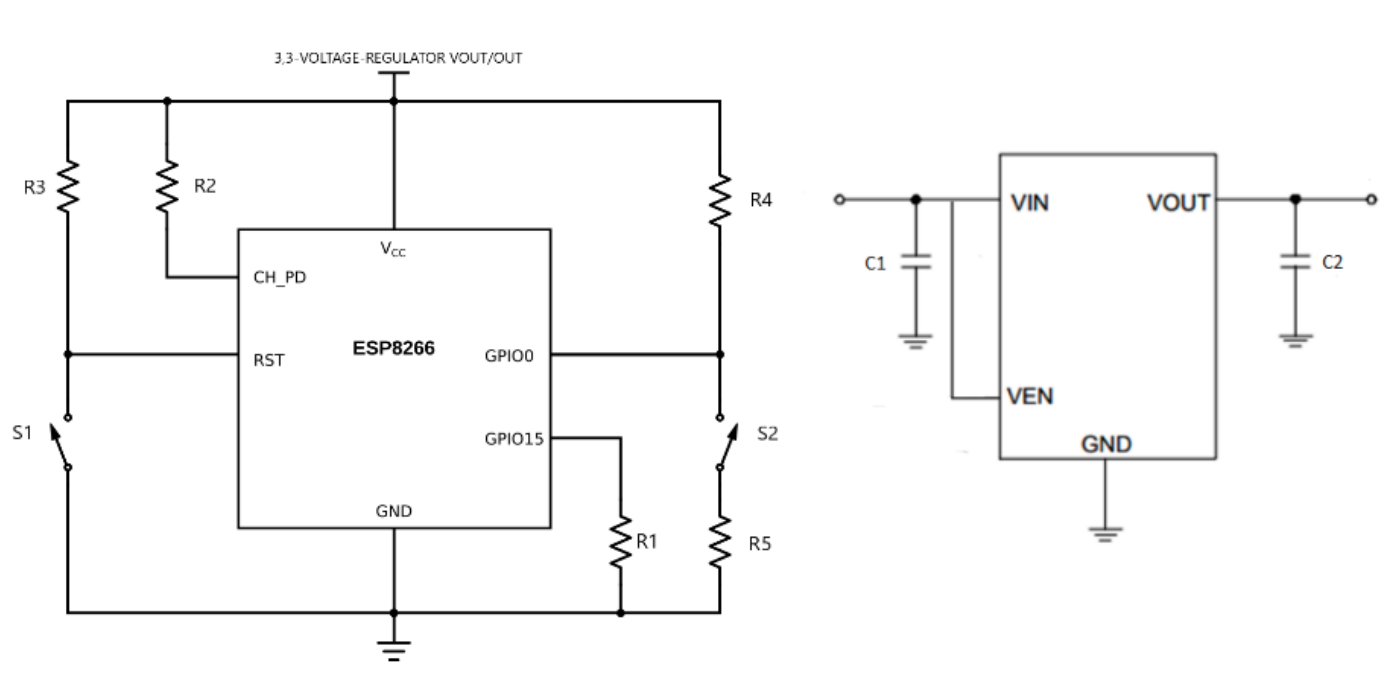
\includegraphics[width=0.8\linewidth]{P1/img/referensi.png}
    \caption{Referensi Rangkaian} 
    \label{fig:referensirangkaian}
\end{figure}

\textbf{Referensi rangkaian:} 
\begin{figure}[H]
    \centering
    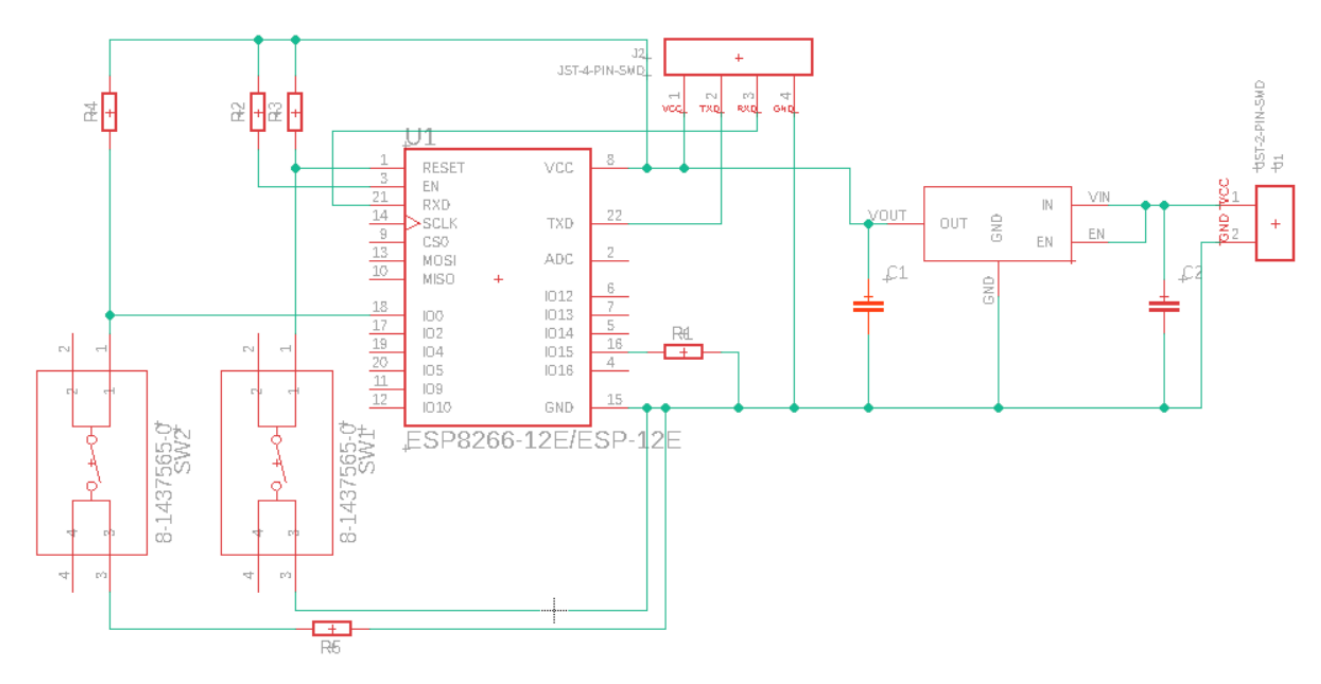
\includegraphics[width=1.1\linewidth]{P1/img/hasiljadischematic.png}
    \caption{Hasil Schematics} 
    \label{fig:hasilschematics}
\end{figure}

\section{Eksperimen 2: Routing Board Minimum System ESP8266}
Setelah proses penyusunan schematic selesai, waktunya mendesain bagaimana board
dari schematic tersebut akan tersusun.
\begin{enumerate}
    \item Untuk melanjutkan mendesain board dari schematic gunakan tools \textbf{“Switch to PCB
    documentation”}
    \begin{figure}[H]
        \centering
        
\includegraphics[width=0.4\linewidth]{P1/img/switchtopcb.png}
        \caption{Tools Switch to PCB} 
        \label{fig:toolsswitchtopcb}
    \end{figure}
    Pada bagian awal saat mengubah ke board, akan disuguhkan tampilan sebagai berikut. Pada
    bagian kiri terdapat Footprint dari komponen dengan garis warna kuning yang
    menghubungkan antar footprint komponen sesuai dengan wiring pada schematic. Pada
    bagian kanan terdapat “Board” yang berbentuk persegi hitam yaitu tempat untuk meletakan
    footprint komponen.
    \begin{figure}[H]
        \centering
        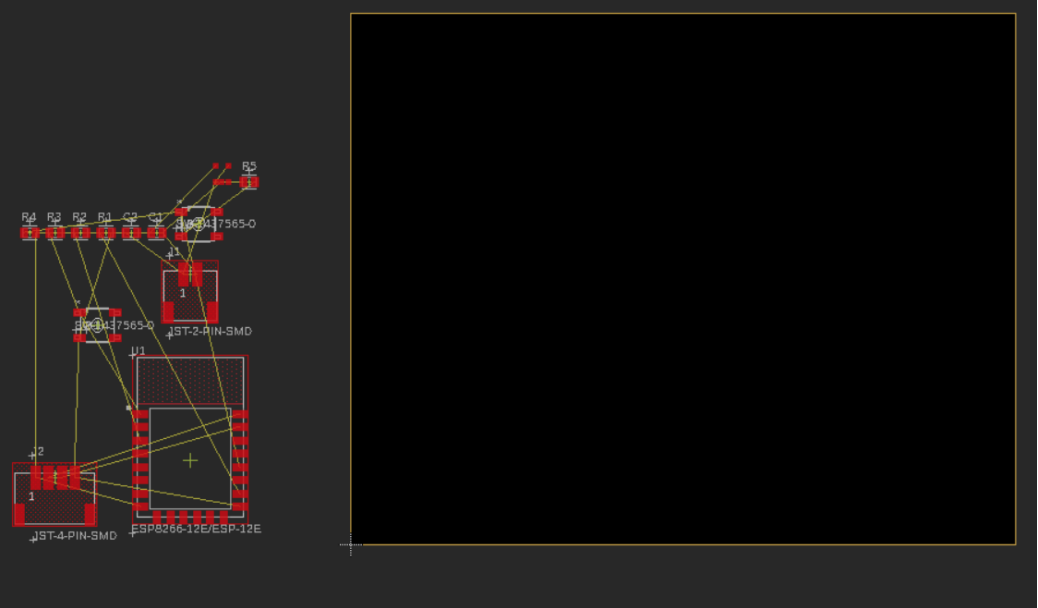
\includegraphics[width=0.9\linewidth]{P1/img/PCBawal.png}
        \caption{Tampilan Awal Board} 
        \label{fig:tampilanawalboard}
    \end{figure}
    \vspace{-\topsep}
    \item Masukan seluruh footprint komponen ke dalam Board dengan memilih seluruh footprint menggunakan tools \textbf{Group} dan digerakan dengan menggukan tools \textbf{Move}.
    \begin{figure}[H]
        \centering
        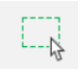
\includegraphics[width=0.15\linewidth]{P1/img/group.png}
        
\includegraphics[width=0.12\linewidth]{P1/img/move.png}
        \caption{Group dan Move}
    \end{figure}
    \begin{figure}[H]
        \centering
        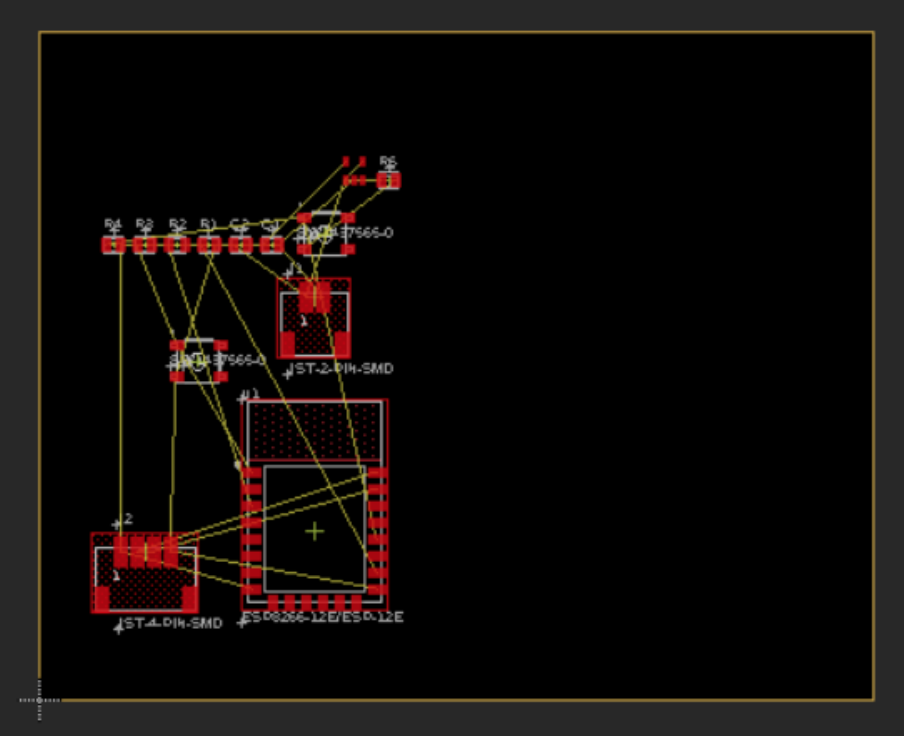
\includegraphics[width=0.7\linewidth]{P1/img/aftermove.png}
        \caption{Hasil Setelah Dipindah}
        \label{fig:hasilsetelahdipindah}
    \end{figure}
    \item Susun footprint serapi mungkin dengan mengerakan footprint menggunakan tools
    \textbf{Move}
    \begin{figure}[H]
        \centering
        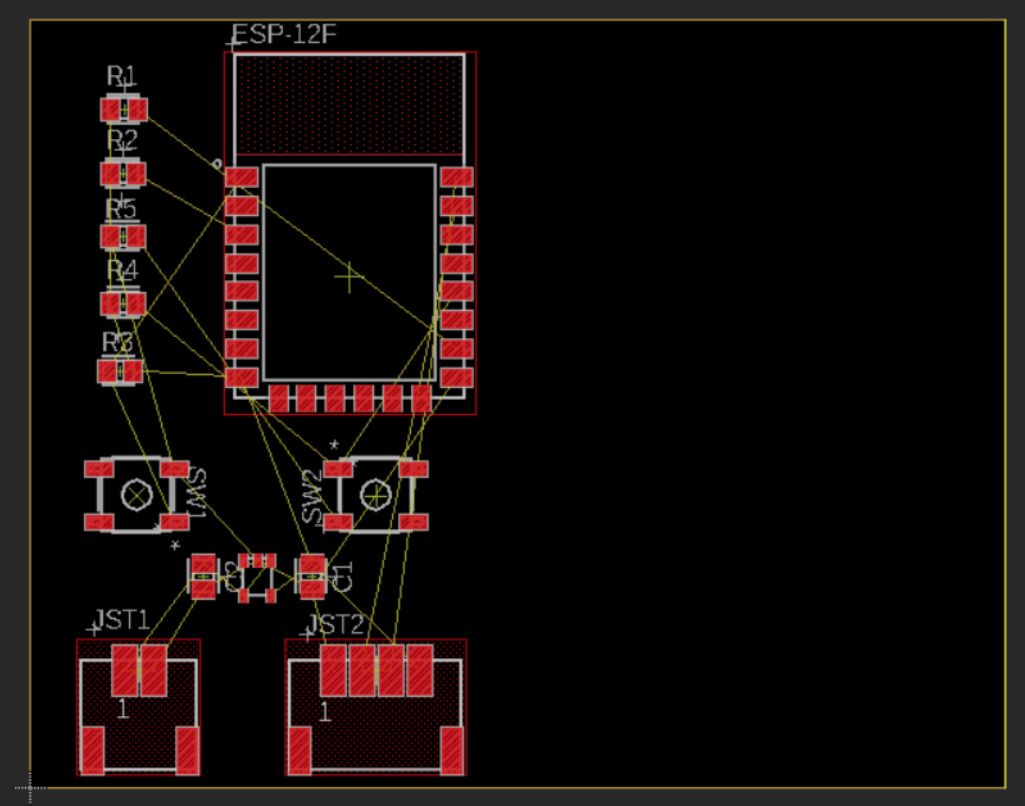
\includegraphics[width=0.7\linewidth]{P1/img/aftermove2.png}
        \caption{Hasil Setelah Dirapikan}
        \label{fig:hasilsetelahdirapikan}
    \end{figure} 
    \item Atur ukuran “Board” dengan menggerakan/geser garis tepi dari “Board” hingga ukuran
    sesuai dengan tatanan footprint.
        \begin{figure}[H]
            \centering
            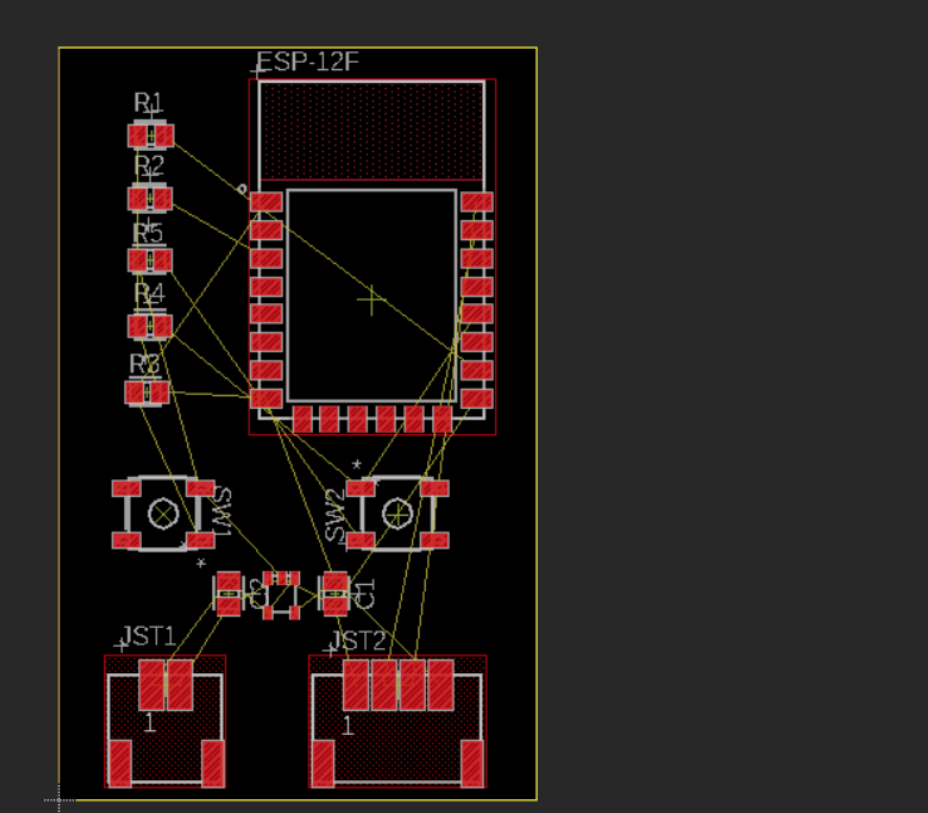
\includegraphics[width=0.7\linewidth]{P1/img/aturukuranboard.png}
        \end{figure}
    \item Selanjutnya adalah melakukan routing jalur koneksi. Dalam melakukan Routing, Tools
    utama yang digunakan adalah \textbf{Route Manual} dan \textbf{Unroute} untuk
    menghapus route. Jalur Routing mengikuti garis warna kuning.
        \begin{figure}[H]
            \centering
            
\includegraphics[width=0.12\linewidth]{P1/img/manualroute.png}
            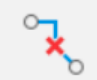
\includegraphics[width=0.17\linewidth]{P1/img/unroute.png}
            \caption{Manual route dan unroute}
        \end{figure}
        \begin{figure}[H]
            \centering
            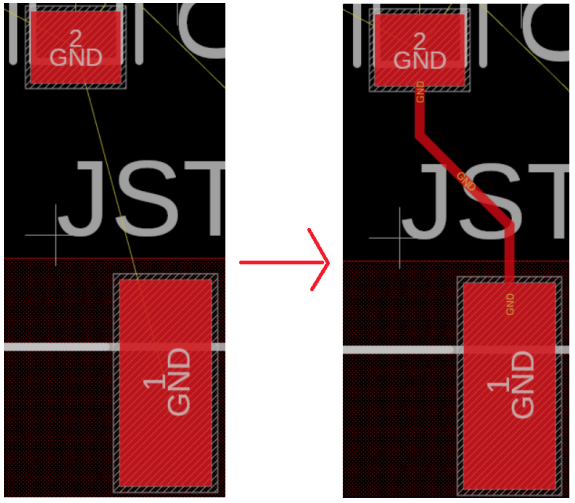
\includegraphics[width=0.89\linewidth]{P1/img/routing1.png}
            \caption{Contoh cara routing}
        \end{figure}
    \item Saat menggunakan Routing normalnya layer yang digunakan adalah \textbf{1 Top} akan tetapi
    Routing yang dibuat di layer yang sama tidak bisa saling ditabrak/ tumpuk.
        \begin{figure}[H]
            \centering
            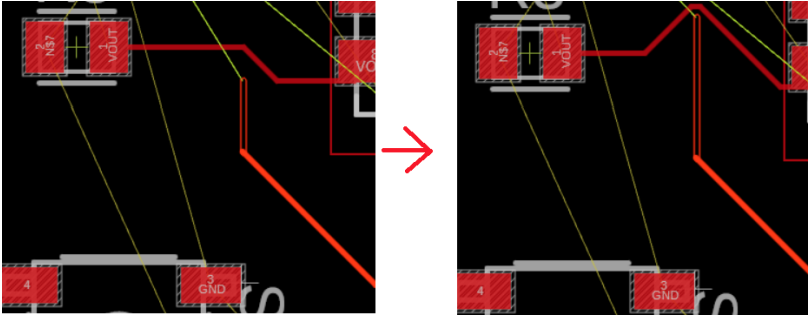
\includegraphics[width=0.89\linewidth]{P1/img/routing2.png}
            \caption{Contoh routing routing yang bertabrakan}
        \end{figure}
    Maka untuk mengatasi hal itu dapat digunakan layer yang lain. Untuk berpindah layer
    menjadi \textbf{16 Bottom} saat menggunakan Route Manual dapat di klik mouse 3 (scroll wheel)
    untuk meletakan \textbf{Vias} yaitu lingkaran penghubung layer top dan bottom. Berpindah layer
    berfungsi agar jalur routing tidak bertabrakan.
        \begin{figure}[H]
            \centering
            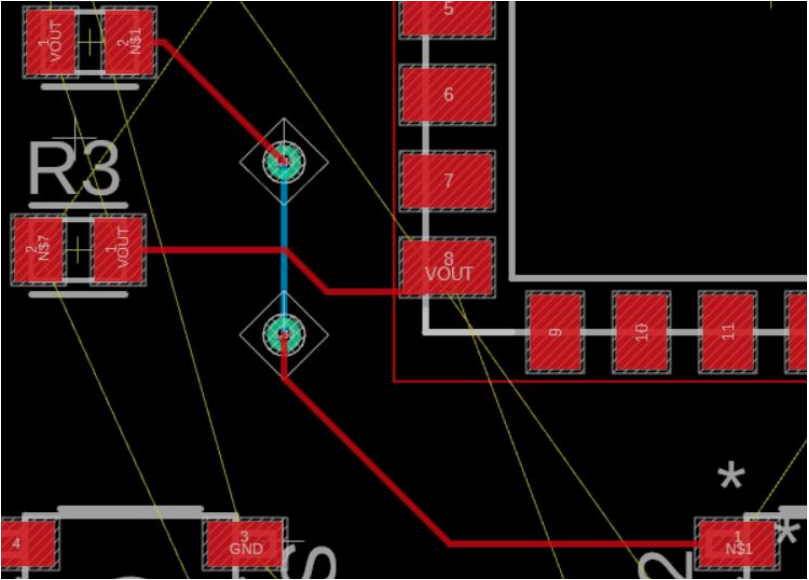
\includegraphics[width=0.89\linewidth]{P1/img/routing3.png}
            \caption{Vias yang menghubungkan Routing top(merah) dengan Bottom(biru)}
        \end{figure}
    \item Routing Seluruh garis koneksi warna kuning hingga seluruhnya tersambung. \textbf{
    Pastikan jalur Routing tidak saling berdekatan dengan jalur lain.}
        \begin{figure}[H]
            \centering
            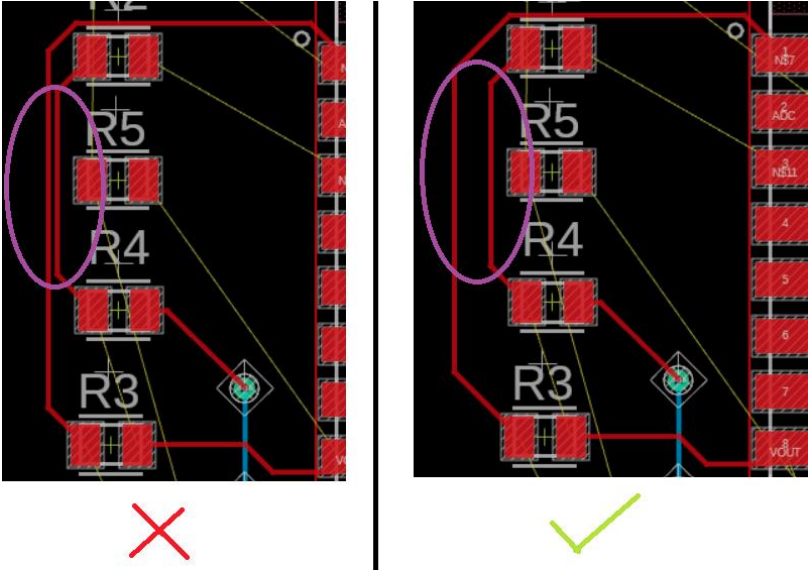
\includegraphics[width=0.89\linewidth]{P1/img/routing4.png}
            \caption{Contoh rangkaian yang tidak bagus dan bagus}
        \end{figure}
\clearpage
    \item Setelah selesai klik save (ctrl+s).
    \textbf{Contoh rangkaian PCB yang sudah jadi :}
        \begin{figure}[H]
            \centering
            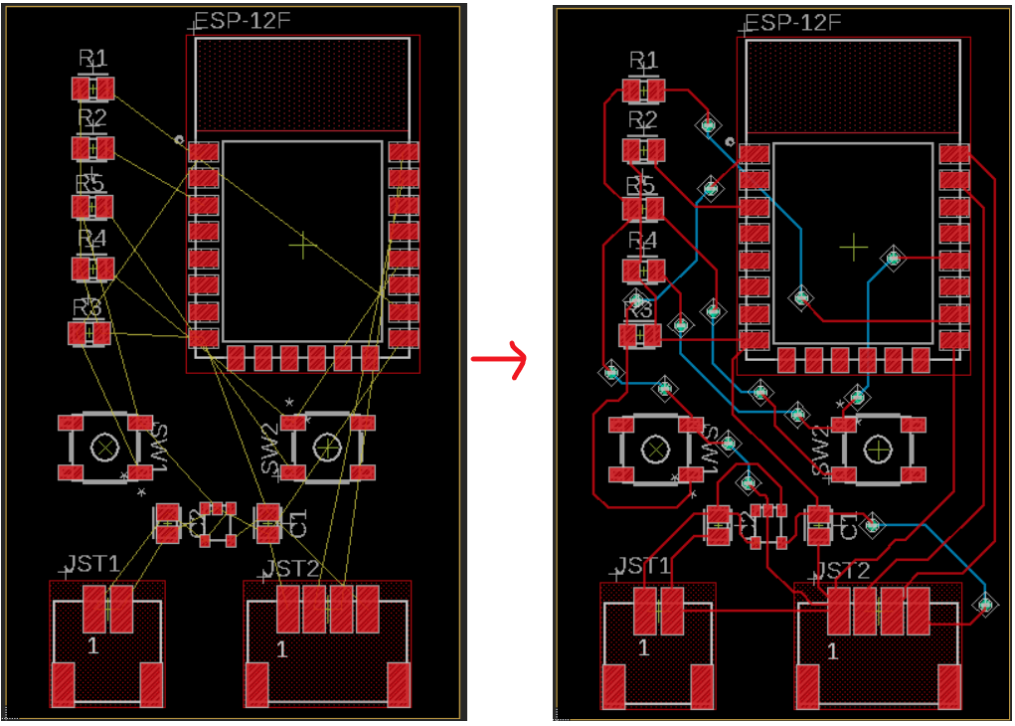
\includegraphics[width=0.89\linewidth]{P1/img/routing5.png}
        \end{figure}
\end{enumerate}